\documentclass{beamer}
\usepackage[utf8]{inputenc}
\usepackage[english]{babel}
\usepackage[labelformat = empty, labelsep = none]{caption}
\usepackage{hyperref}

%\usetheme{AnnArbor}
%\usetheme{Antibes}
%\usetheme{Bergen}
%\usetheme{Berkeley}
%\usetheme{Berlin}
%\usetheme{CambridgeUS}
%\usetheme{Copenhagen}
%\usetheme{Darmstadt}
%\usetheme{Dresden}
%\usetheme{Frankfurt}
%\usetheme{Goettingen}
%\usetheme{Hannover}
%\usetheme{Ilmenau}
%\usetheme{JuanLesPins}
%\usetheme{Luebeck}
\usetheme{Madrid}
%\usetheme{Malmoe}
%\usetheme{Marburg}
%\usetheme{Montpellier}
%\usetheme{PaloAlto}
%\usetheme{Pittsburgh}
%\usetheme{Rochester}
%\usetheme{Singapore}
%\usetheme{Szeged}
%\usetheme{Warsaw}
%\usetheme{boxes}
%\usetheme{default}
%\usecolortheme{default}
%\usecolortheme{albatross}
\usecolortheme{beaver}
%\usecolortheme{beetle}
%\usecolortheme{crane}
%\usecolortheme{dolphin}
%\usecolortheme{dove}
%\usecolortheme{fly}
%\usecolortheme{lily}
%\usecolortheme{orchid}
%\usecolortheme{rose}
%\usecolortheme{seagull}
%\usecolortheme{seahorse}
%\usecolortheme{whale}
%\usecolortheme{wolverine}
\hypersetup{colorlinks=true, linkcolor=blue, filecolor=magenta, urlcolor=cyan}
\urlstyle{same}

\title{Amateur Telescope Making}
\subtitle{...or how to make your own telescope at home}
\author{Nuno Miguel Sousa}
\institute{Coimbra, Portugal}
\date{\today}


\begin{document}

\begin{frame}
\titlepage
\end{frame}

\begin{frame}
\frametitle{What is Amateur Telescope Making?}
\begin{block}{}
Amateur Telescope Making, or ATM, is a hobby taken by people that have an interest in astronomic observation and enjoy building telescopes.\footnotemark
\end{block}
\footnotetext{\url{https://en.wikipedia.org/wiki/Amateur_telescope_making}}
\begin{block}{}
ATM can range from just assembling the individually bought components to actually fabricate some or all of the components of a telescope.
\end{block}
\begin{block}{}
The most common type of telescope made by hobbyists is the so called Newtonian reflector (invented by Sir Isaac Newton).\footnotemark
\end{block}
\footnotetext{\url{https://en.wikipedia.org/wiki/Newtonian_telescope}}
\end{frame}

\begin{frame}
\frametitle{My personal motivation for ATM}
\begin{columns}
\column{0.6\textwidth}
One time by chance a few years ago, I had the opportunity to look up at the night sky in Alentejo's countryside, in southern Portugal.

The combination of very low light pollution and clear sky provided for a very distinctive view of the Milky Way.

I had some interest in astronomy in general, but that event was what sparked the beginning of my interest in astronomical observation.

Eventually I found about ATM and ended up deciding to build a telescope myself because I found the challenge interesting.
\column{0.4\textwidth}
\begin{figure}
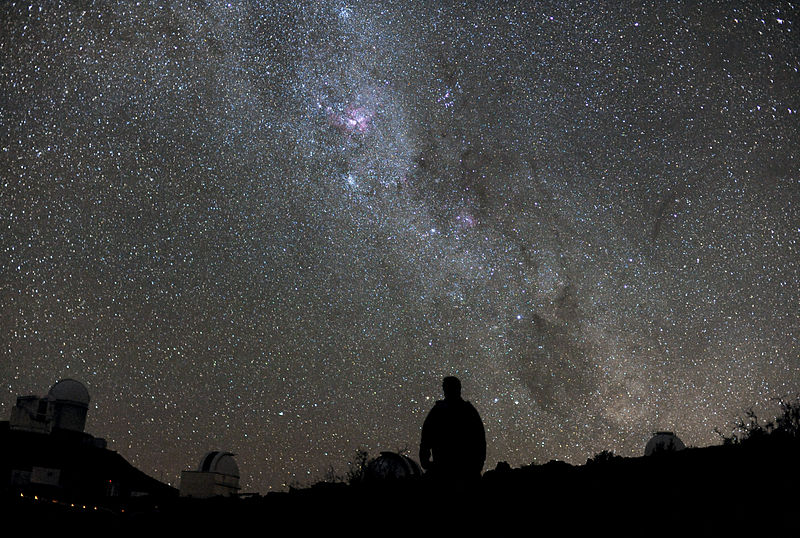
\includegraphics[scale=0.45]{assets/800px-Starry_Night_at_La_Silla.jpg}
\caption{Not me!}
\end{figure}
\end{columns}
\end{frame}

\begin{frame}
\frametitle{What I'm working on?}
I'm building a Newtonian reflector telescope and I'm making the main mirror lens myself.

It has a 200mm diameter main mirror and initially I planned for a focal length of 1200mm.

Why these choices?
\begin{itemize}
\item For a certain telescope diameter (aperture), it is the least complicated type to make (only one convex main mirror lens and a small diagonal flat mirror).
\item A 200mm main mirror with 1200mm focal length is one of the most common configurations. It is a compromise between portability and light collection capability.
\item Provided you make some simple tools, the mirror's optical quality will only be limited by the amount of time you want to spend and patience (or lack thereof).
\end{itemize}
\end{frame}

\begin{frame}
\frametitle{The Newtonian Reflector telescope}
\begin{figure}
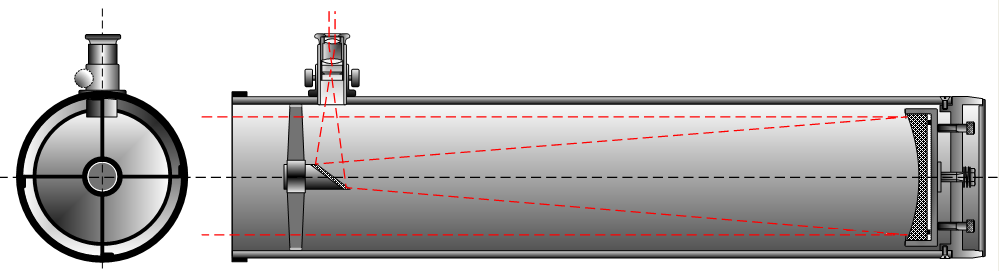
\includegraphics[scale=0.4]{assets/Newtontelescope.png}
\caption{Newtonian telescope}
\end{figure}
The main components of a Newtonian reflector telescope are the main concave mirror\footnotemark,\footnotetext{\url{https://en.wikipedia.org/wiki/Primary_mirror}}
the diagonal flat mirror, and the eyepiece\footnotemark.
\footnotetext{\url{https://en.wikipedia.org/wiki/Eyepiece}}

Incoming light (red dashed line) comes from the top of the telescope, illuminates the main mirror, and is reflected back to the eyepiece by the diagonal mirror.
\end{frame}

\begin{frame}
\frametitle{Making the main mirror}
In a good mirror, its surface must not have any imperfections with more than $0.07 \mu m$ of deviation from the theoretical ideal surface.
This ideal surface must be a paraboloid\footnotemark to correctly focus the light rays coming from very far away objects.
\footnotetext{\url{https://en.wikipedia.org/wiki/Parabolic_reflector}}

How does one make such smooth surface? It turns out it can be done with easily built hand tools and a simple set of steps:

\begin{itemize}
\item \textit{Rough grinding}. Generates a first approximation of the optical surface. Results in a rough surface.
\item \textit{Fine grinding and smoothing}. Removes all the major pits and scratches created in rough grinding and further approximates the optical surface.
\item \textit{Polishing}. Complete removal of small pits and scratches.
\item \textit{Testing and retouching}. Examination of the mirror for defects and their correction.
\end{itemize}
\end{frame}

\begin{frame}
\frametitle{Mirror grinding and smoothing}
\begin{columns}
\column{0.5\textwidth}
Mirror grinding and smoothing operations are accomplished with a tool and a sequence of abrasives. The set of abrasives goes from very coarse ($0.1mm$) during initial rough grinding to very fine ($10 \mu m$) on the later stages of smoothing.

The tool must be a disc with similar size to that of the mirror. It can be made of glass or other hard material.

Variations of a W movement are performed between tool and mirror disc while also stepping from position to position around the mirror.
\column{0.5\textwidth}
\begin{figure}
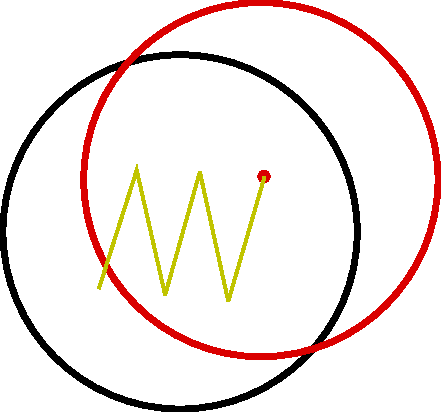
\includegraphics[scale=0.35]{assets/stroke.pdf}
\end{figure}
\begin{figure}
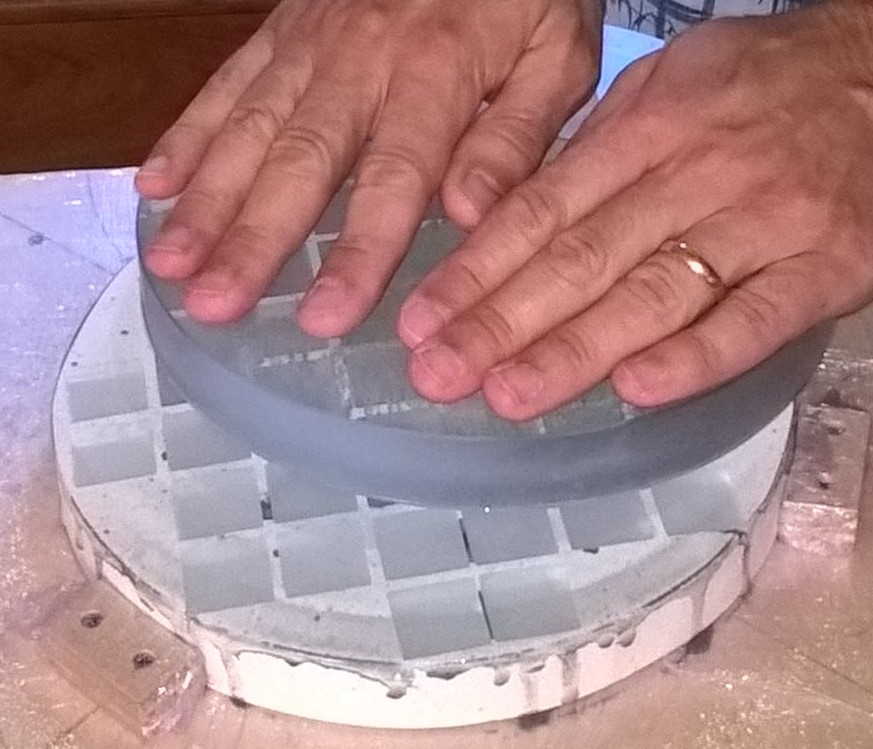
\includegraphics[scale=0.2]{assets/grinding.jpg}
\end{figure}
\end{columns}
\end{frame}

\begin{frame}
\frametitle{Mirror polishing}
\begin{columns}
\column{0.5\textwidth}
Mirror polishing is accomplished with a softer substrate applied to the tool's surface (usually optical pitch) and a very fine ($<1 \mu m$) polishing abrasive.

Polishing is performed with a similar set of W movements as used in smoothing.
\column{0.5\textwidth}
\begin{figure}
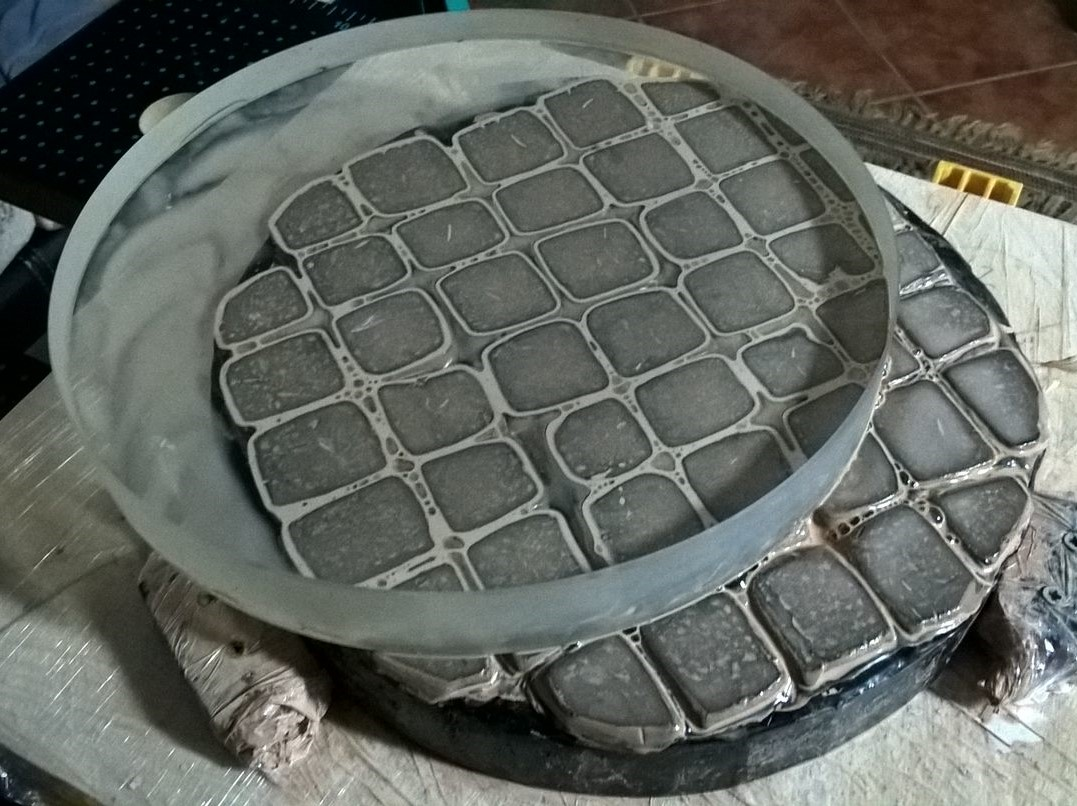
\includegraphics[scale=0.2]{assets/polishing.jpg}
\end{figure}
\end{columns}
\end{frame}

\begin{frame}
\frametitle{Mirror testing}
After having produced a curve of the proper depth and having removed any signs of scratches or pits, it is time to test the mirror's surface.

The purpose of testing is to examine how close to the ideal curve the actual mirror is and to plan how to correct it.

There are several tests that can be used with varying degrees of complexity and information produced.
\begin{itemize}
\item \textit{Ronchi test}. Produces mainly qualitative results. Of limited use.
\item \textit{Foucault test}. Produces quantitative results but is not very sensitive to non-figure of revolution defects.
\item \textit{Interferometry test}. Produces the best quantitative results. Gives a topographical error of the mirror's surface.
\end{itemize}
\end{frame}

\begin{frame}
\frametitle{Foucault test}
\begin{columns}
\column{0.5\textwidth}
The Foucault test is one of the oldest types of test available to the amateur to test their mirror.

It is the most popular test within the ATM circle. This is due both to its ease of understanding and operation\footnote[frame]{\url{https://atm-workshop.com/foucault.html}}, and also because the tester hardware is easy to build from commonly obtainable materials\footnote[frame]{\url{https://stellafane.org/stellafane-main/tm/atm/test/tester-1.html}}.
\column{0.5\textwidth}
\begin{figure}
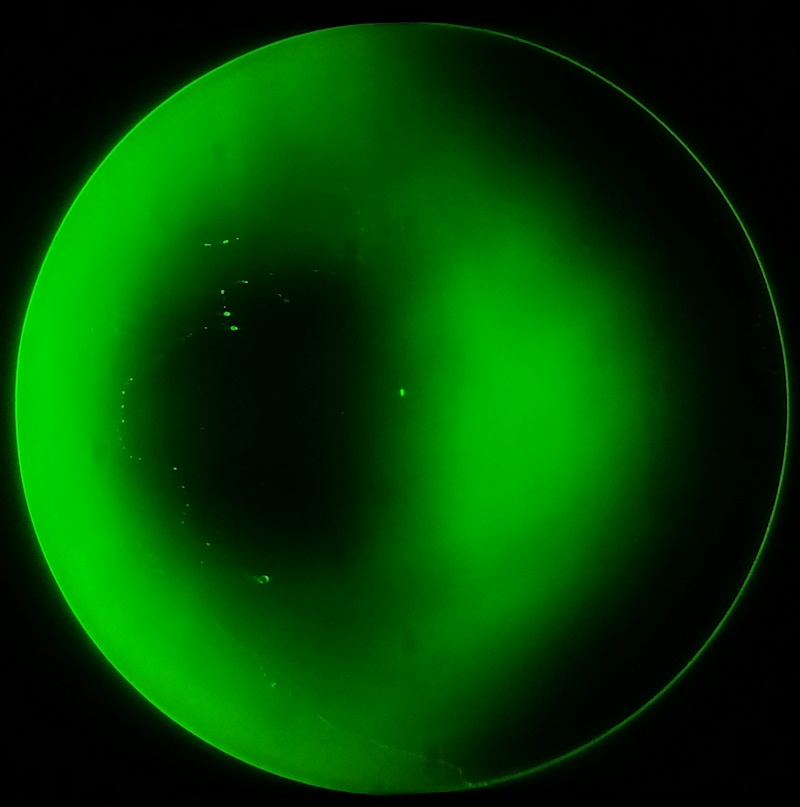
\includegraphics[scale=0.3]{assets/Foucault.jpg}
\caption{Foucault test capture during actual testing on my mirror. This capture is one of a series of captures taken at specific offsets from the mirror's radius of curvature.}
\end{figure}
\end{columns}
\end{frame}

\begin{frame}
\frametitle{Interferometry test}
\begin{columns}
\column{0.5\textwidth}
Interferometry testing is a much more recent addition to the ATM tool set.

The availability of cheap solid state laser diodes and a few optical components, made possible for a simplified interferometer called the Bath Interferometer to be build at home\footnote[frame]{\url{http://rohr.aiax.de/Using a Bath - EN.pdf}}. Coupled with open source software made by the ATM community provided for a complete solution to perform interferometry analysis.
\column{0.5\textwidth}
\begin{figure}
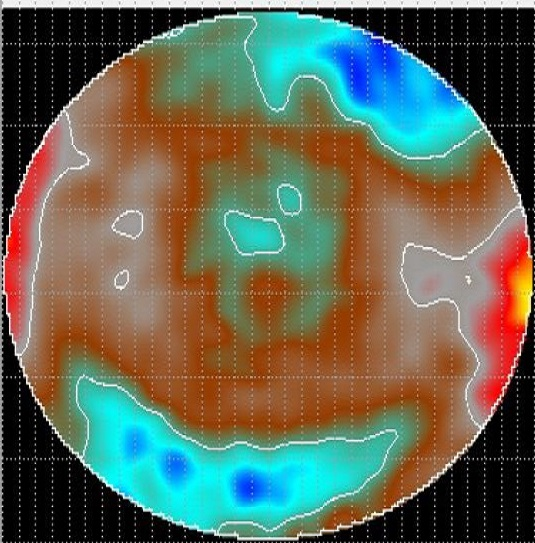
\includegraphics[scale=0.3]{assets/bath.jpg}
\caption{This report shows the actual defects present on my mirror's surface relative to the ideal surface. In this case the mirror shows some astigmatism seen by its potato chip like error shape.}
\end{figure}
\end{columns}
\end{frame}


\begin{frame}
\frametitle{Current state and next steps}
So far I have only worked on the mirror lens and it has been a very interesting learning experience.

As shown in the previous slide, the mirror is showing some astigmatism defects that need to be resolved. This is the current state.

After that, the next step will be to have it electrically coated with a very thin aluminum reflective coating. I can't do this myself, so I need to send it over to a specialized facility to do that for me.

When the mirror is done, what remains to be built is the Optical Tube Assembly (OTA). I will build the tube myself, but will buy the remaining components, like the mirror cell, the focuser and the diagonal mirror.
\end{frame}

\begin{frame}
\frametitle{About the author}
My name is Nuno Sousa and I'm from Peniche, Portugal.

I graduated in Electrical Engineering an have a general interest in science.

I was welcomed into the the Critical family 6 years ago and I've been working mainly in the aviation industry.

I like science fiction, to build stuff, specially electronic circuits and of course the telescope I was talking about.

\begin{figure}
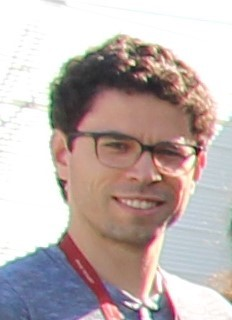
\includegraphics[scale=0.3]{assets/self.jpg}
\end{figure}
\end{frame}

\begin{frame}
\frametitle{The end}
\centering
Thank you!
\end{frame}

\end{document}
